%!TEX spellcheck
%!TEX root = ../bachelor_paper.tex
\documentclass[../bachelor_paper.tex]{subfiles}
\graphicspath{{\subfix{images/}}}
\begin{document}

\chapter{Temporal analysis graphs of all measured applications}
    \label{ch:graphs}

% Coremark   
\begin{figure}
    \begin{subfigure}{0.45\textwidth}
        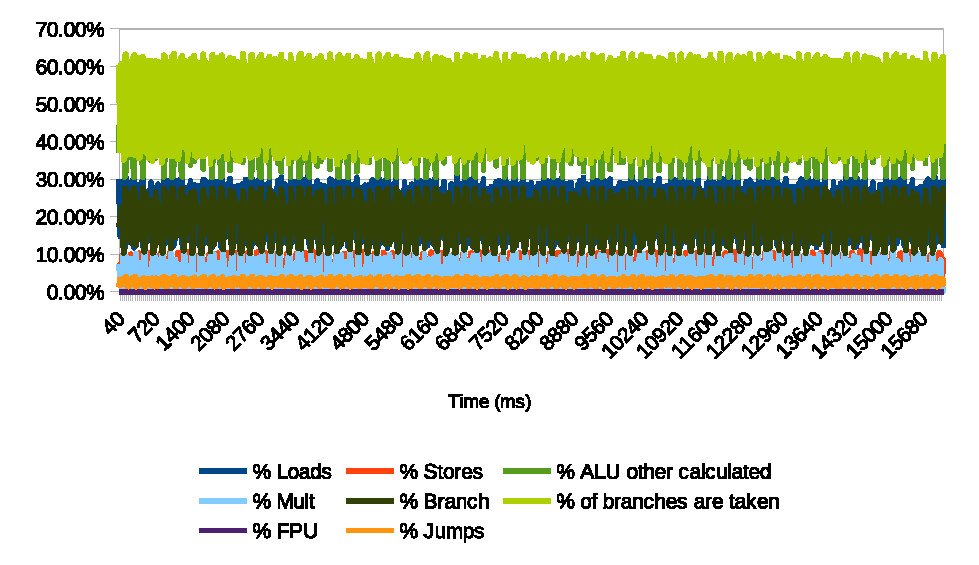
\includegraphics[width=\textwidth]{img/graph/coremark/coremark_inst.eps}
        \caption{Instruction behavior over time (ms)}
    \end{subfigure}
    \begin{subfigure}{0.45\textwidth}
        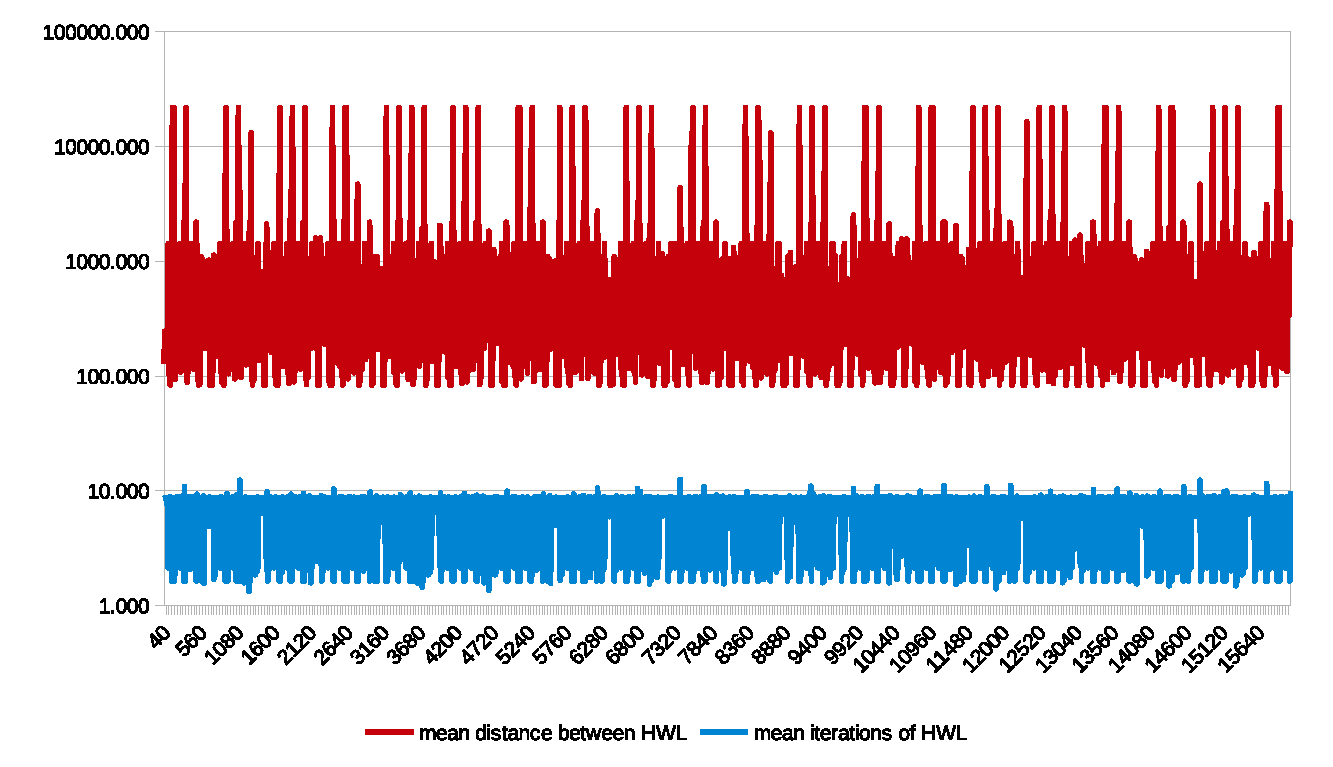
\includegraphics[width=\textwidth]{img/graph/coremark/coremark_hwl.eps}
        \caption{\ac{HWL} behavior over time (ms)}
    \end{subfigure}
    \begin{subfigure}{0.45\textwidth}
        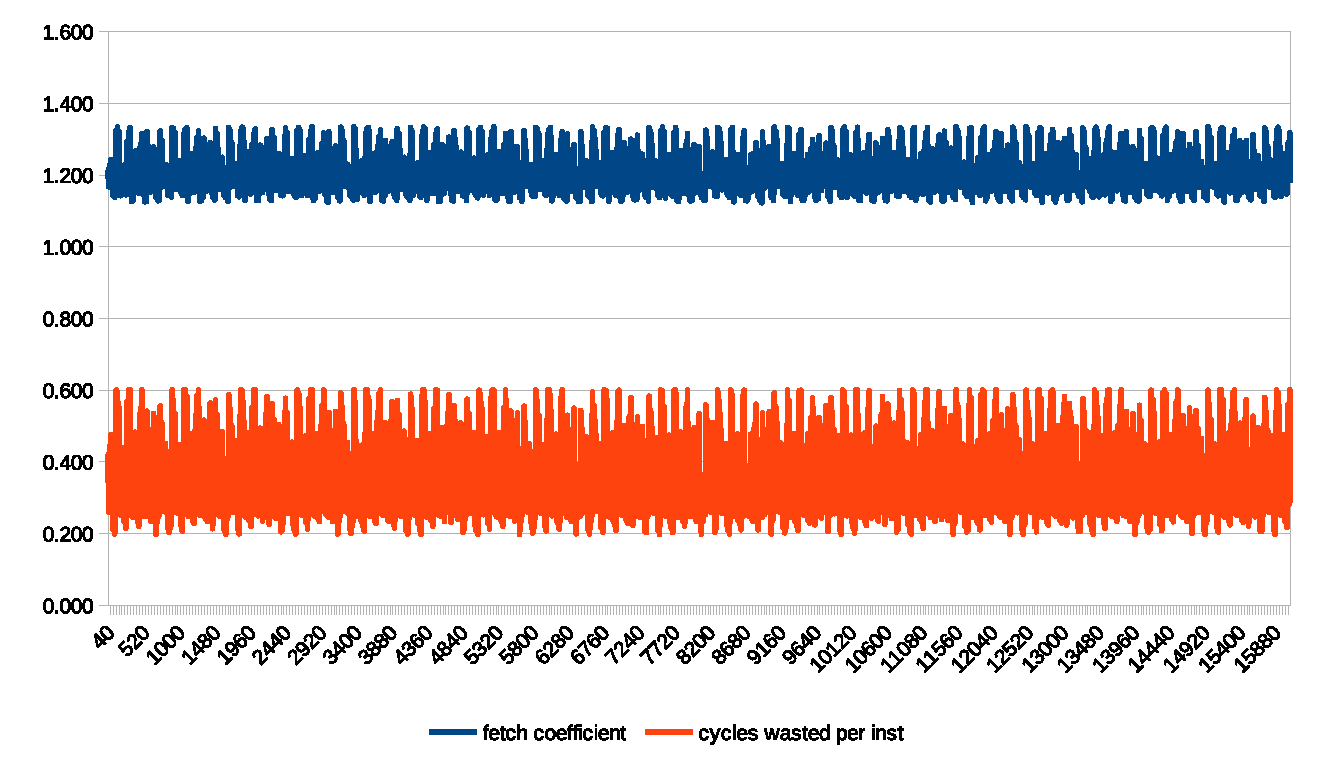
\includegraphics[width=\textwidth]{img/graph/coremark/coremark_fetch_waste.eps}
        \caption{Fetch coefficient and cycles wasted per instruction over time (ms)}
    \end{subfigure}
    \caption{Coremark}
\end{figure}

%%%%%%%%% MIBENCH %%%%%%%%%
% basicmath   
\begin{figure}
    \begin{subfigure}{0.45\textwidth}
        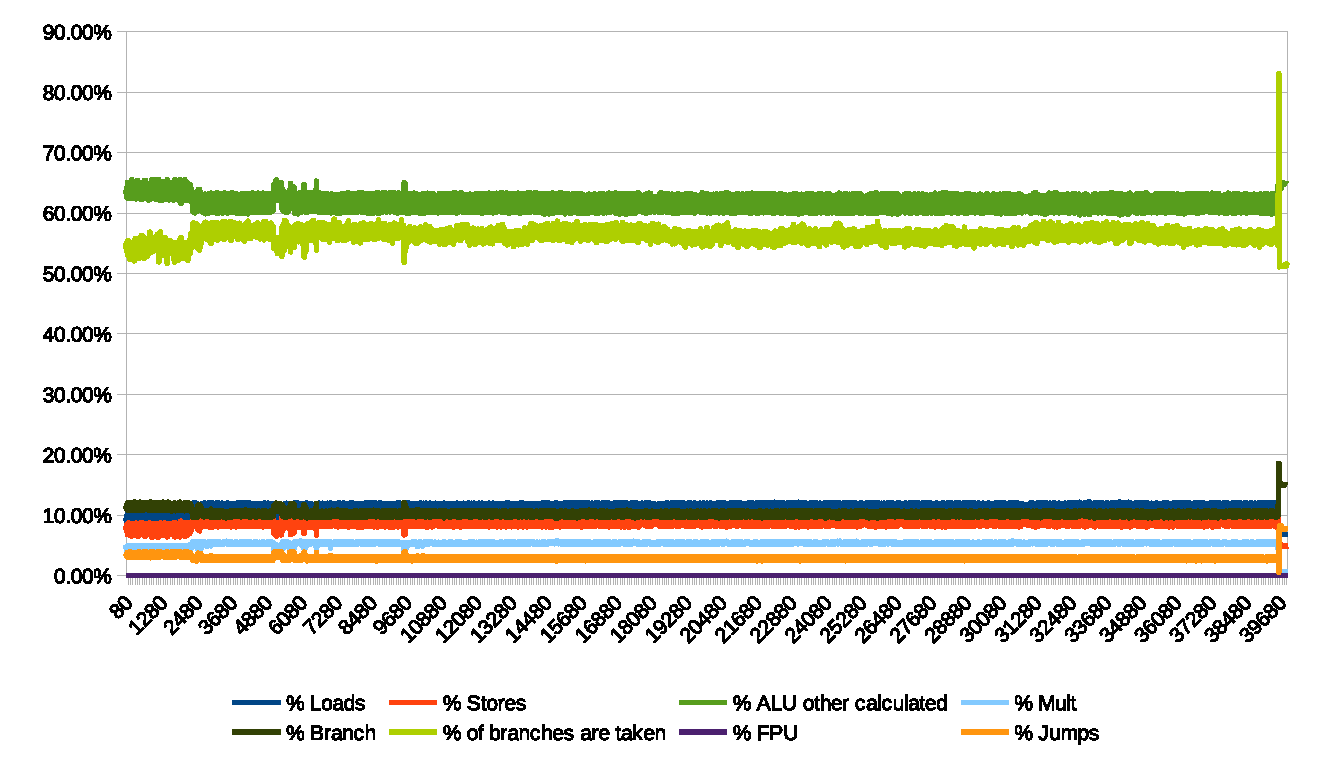
\includegraphics[width=\textwidth]{img/graph/mibench/basicmath_inst.eps}
        \caption{Instruction behavior over time (ms)}
    \end{subfigure}
    \begin{subfigure}{0.45\textwidth}
        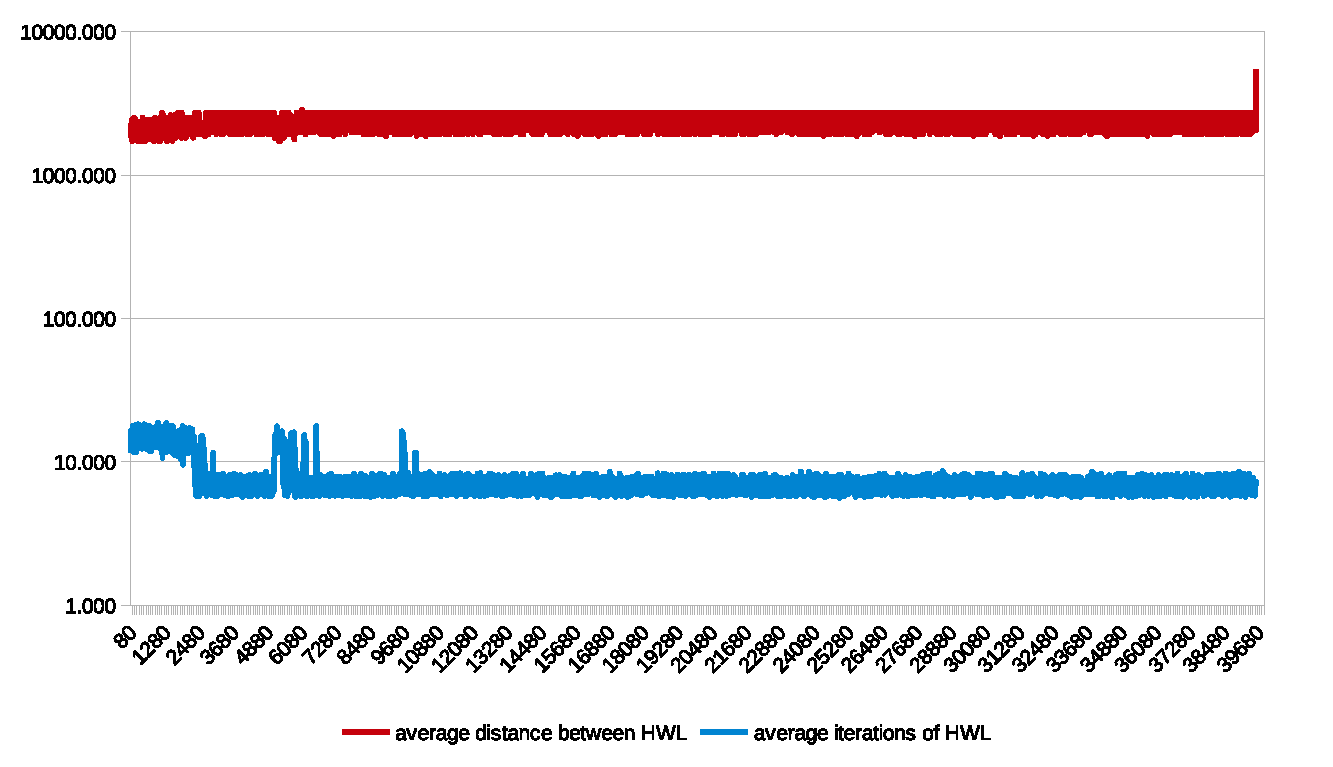
\includegraphics[width=\textwidth]{img/graph/mibench/basicmath_hwl.eps}
        \caption{\ac{HWL} behavior over time (ms)}
    \end{subfigure}
    \begin{subfigure}{0.45\textwidth}
        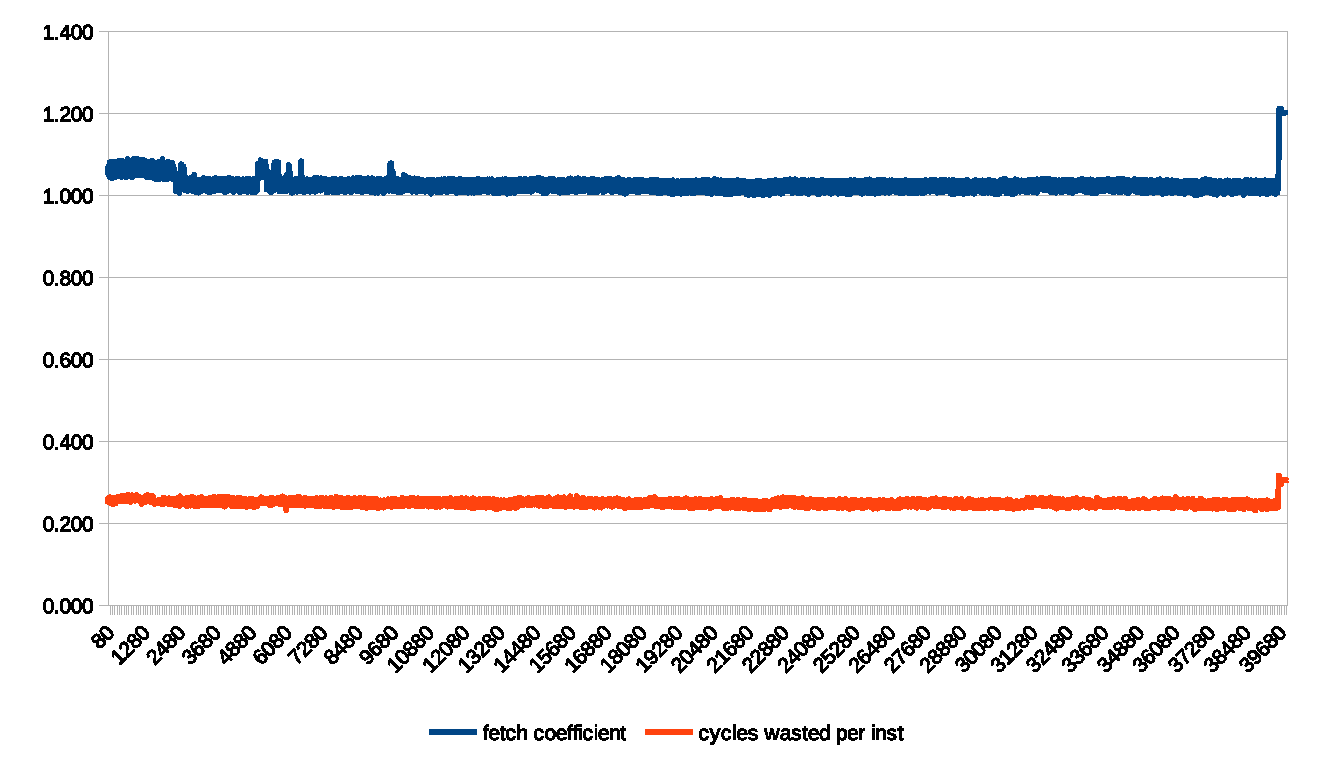
\includegraphics[width=\textwidth]{img/graph/mibench/basicmath_fetch_waste.eps}
        \caption{Fetch coefficient and cycles wasted per instruction over time (ms)}
    \end{subfigure}
    \caption{\texttt{basicmath}}
\end{figure}

% Render bibliograhy and acronyms if rendered standalone
\isstandalone
\bibliographystyle{IEEEtran}
\bibliography{bibliography}
\subfile{abbreviations.tex}
\fi

\end{document} 
